% Options for packages loaded elsewhere
\PassOptionsToPackage{unicode}{hyperref}
\PassOptionsToPackage{hyphens}{url}
%
\documentclass[
]{article}
\usepackage{lmodern}
\usepackage{amssymb,amsmath}
\usepackage{ifxetex,ifluatex}
\ifnum 0\ifxetex 1\fi\ifluatex 1\fi=0 % if pdftex
  \usepackage[T1]{fontenc}
  \usepackage[utf8]{inputenc}
  \usepackage{textcomp} % provide euro and other symbols
\else % if luatex or xetex
  \usepackage{unicode-math}
  \defaultfontfeatures{Scale=MatchLowercase}
  \defaultfontfeatures[\rmfamily]{Ligatures=TeX,Scale=1}
\fi
% Use upquote if available, for straight quotes in verbatim environments
\IfFileExists{upquote.sty}{\usepackage{upquote}}{}
\IfFileExists{microtype.sty}{% use microtype if available
  \usepackage[]{microtype}
  \UseMicrotypeSet[protrusion]{basicmath} % disable protrusion for tt fonts
}{}
\makeatletter
\@ifundefined{KOMAClassName}{% if non-KOMA class
  \IfFileExists{parskip.sty}{%
    \usepackage{parskip}
  }{% else
    \setlength{\parindent}{0pt}
    \setlength{\parskip}{6pt plus 2pt minus 1pt}}
}{% if KOMA class
  \KOMAoptions{parskip=half}}
\makeatother
\usepackage{xcolor}
\IfFileExists{xurl.sty}{\usepackage{xurl}}{} % add URL line breaks if available
\IfFileExists{bookmark.sty}{\usepackage{bookmark}}{\usepackage{hyperref}}
\hypersetup{
  pdftitle={Biophysical Modeling: a Primer with LANDFIRE},
  hidelinks,
  pdfcreator={LaTeX via pandoc}}
\urlstyle{same} % disable monospaced font for URLs
\usepackage[margin=1in]{geometry}
\usepackage{graphicx}
\makeatletter
\def\maxwidth{\ifdim\Gin@nat@width>\linewidth\linewidth\else\Gin@nat@width\fi}
\def\maxheight{\ifdim\Gin@nat@height>\textheight\textheight\else\Gin@nat@height\fi}
\makeatother
% Scale images if necessary, so that they will not overflow the page
% margins by default, and it is still possible to overwrite the defaults
% using explicit options in \includegraphics[width, height, ...]{}
\setkeys{Gin}{width=\maxwidth,height=\maxheight,keepaspectratio}
% Set default figure placement to htbp
\makeatletter
\def\fps@figure{htbp}
\makeatother
\setlength{\emergencystretch}{3em} % prevent overfull lines
\providecommand{\tightlist}{%
  \setlength{\itemsep}{0pt}\setlength{\parskip}{0pt}}
\setcounter{secnumdepth}{-\maxdimen} % remove section numbering

\title{Biophysical Modeling: a Primer with LANDFIRE}
\author{}
\date{\vspace{-2.5em}}

\begin{document}
\maketitle

\hypertarget{what-will-you-find-on-this-website}{%
\subsubsection{What will you find on this
website?}\label{what-will-you-find-on-this-website}}

Brief tutorials on how to use BpS models and the free modeling software,
SyncroSim. When integrated into state and transition models, this
framework can improve and enhance landscape predictions and research
projections.

LANDFIRE's state-and-transition simulation models use inputs such as the
rates of growth and the probabilities of different disturbances to
simulate the dynamics of ecosystem over time. LANDFIRE uses the models
to estimate the historical composition and structure of ecosystems and
the frequency and severity of wildfire prior to European-American
settlement, but they can be used for a variety of other purposes.

What is a biophysical model?\\
Bps models use quantative simulations of biological and physical inputs
to make predictions about the future of natural systems. LANDFIRE's BpS
models were created using state and transition models to summarize
ecosystem processes such as \textbf{growth rates} and
\textbf{disturbance probabilities} while simulating their dynamic
interplay over time.

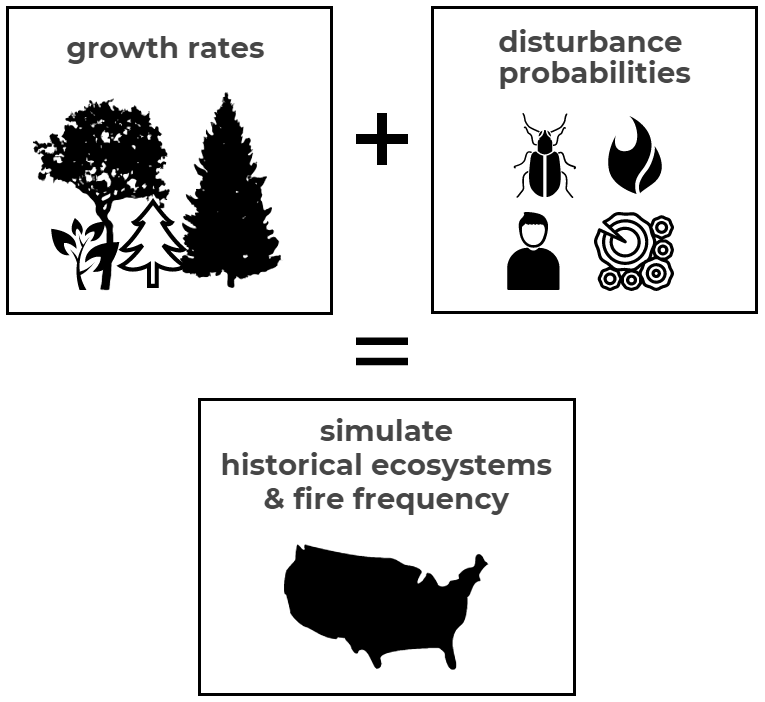
\includegraphics{images/inputmodel.png}

\hypertarget{why-model}{%
\subsubsection{Why model?}\label{why-model}}

\hypertarget{modeling-biophysical-models-provide-a-framework-for}{%
\paragraph{Modeling biophysical models provide a framework
for:}\label{modeling-biophysical-models-provide-a-framework-for}}

\begin{enumerate}
\def\labelenumi{\arabic{enumi}.}
\tightlist
\item
  simulating disturbances and testing potential management strategies\\
\item
  modeling vegetation characteristics on the landscape\\
\item
  making predictions of future landscape conditions
\end{enumerate}

\begin{quote}
Get started with integrating biophysical settings into your current work
\end{quote}

\hypertarget{section}{%
\subsection{}\label{section}}

\end{document}
